\section{Discussion}
\label{sec:discussion}
  Dans cette section, nous revenons sur les résultats présentés dans la
  section~\ref{sec:experiences} et pointons, pour les différentes disciplines,
  les variations qui, selon nous, influent sur la difficulté de la tâche
  d'extraction de termes-clés en domaines de spécialité. À partir des résultats
  obtenus, nous déduisons l'échelle de difficulté suivante (de la discipline la
  plus difficile à la plus facile)~:
  \begin{figure}[h!]
    \centering
    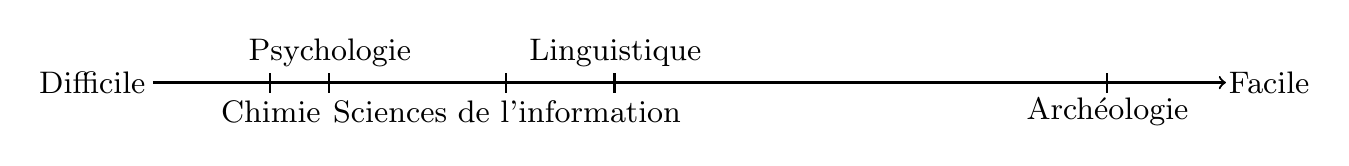
\begin{tikzpicture}[thin,
                        align=center,
                        scale=1.25,
                        every node/.style={text centered, transform shape}]
      \coordinate (start) at (4.5, 0);
      \coordinate (c) at (5.7, 0);
      \coordinate (p) at (6.3, 0);
      \coordinate (s) at (8.1, 0);
      \coordinate (l) at (9.2, 0);
      \coordinate (a) at (14.2, 0);
      \coordinate (end) at (15.4, 0);
      \node (chimie) at (5.7, -0.3) {\small Chimie};
      \node (psychologie) at (6.3, 0.3) {\small Psychologie};
      \node (sciences_de_l_information) at (8.1, -0.3) {\small Sciences de l'information};
      \node (linguistique) at (9.2, 0.3) {\small Linguistique};
      \node (archeologie) at (14.2, -0.3) {\small Archéologie};
      \draw[-|, thick] (start) node[xshift=-1.75em] (dificile) {\small Difficile} -- (c);
      \draw[-|, thick] (c) -- (p);
      \draw[-|, thick] (p) -- (s);
      \draw[-|, thick] (s) -- (l);
      \draw[-|, thick] (l) -- (a);
      \draw[->, thick] (a) -- (end) node[xshift=1.25em] (facile) {\small Facile};
    \end{tikzpicture}
    \caption{
             \label{fig:}}
  \end{figure}
  Selon cette échelle de difficulté, ainsi que selon nos observations du contenu
  des notices, nous définissons trois catégories pour lesquelles la difficulté
  n'est pas la même~:
  \begin{enumerate}
    \item{Travaux expérimentaux (Chimie)}
    \item{Travaux analytiques (Psychologie, Linguistique et Sciences de
          l'Information)}
    \item{Travaux pratiques, i.e.~fondés sur des faits non sujets à subjectivité
          (Archéologie)}
  \end{enumerate}
  \TODO{discuter plus ces catégories}

  Dans un premier temps, nous constatons que l'usage d'une pondération fondée
  sur la spécificité d'un mot vis-à-vis du document
  peut améliorer\TODO{stabiliser?} la performance des méthodes d'extraction de termes-clés. Nous
  en déduisons que la nature linguistique des termes utilisés dans une
  discipline est un facteur influant sur la difficulté de l'extraction des
  termes-clés pour cette même discipline. Ainsi, une forte tendance à l'usage de
  composés syntagmatiques constitués de mots généraux dans la discipline, tels
  que \og{}réaction\fg{} qui est présent dans le terme-clé \og{}réaction
  topotactique\fg{} en Chimie, augmente la difficulté de l'extraction des
  termes-clés.

  Dans un second temps, nous constatons que la capacité à créer des liens entre
  différentes unités textuelles peut aider lors de l'extraction des termes-clés.
  Après observation du contenu des notices, nous remarquons que l'organisation
  du discours du résumé dans les différentes disciplines est un second facteur
  influant sur la difficulté de la tâche d'extraction de termes-clés. Pour
  chaque discipline, le lecteur visé n'est pas le même et le résumé est donc
  organisé différemment. Dans le cas de documents se basant sur des faits
  concrets, tels que les documents d'Archéologie, le lecteur (archéologue ou
  non) a besoin d'une définition du contexte et des relations entre les faits
  donnés. Un document insistant sur différents éléments importants et créant des
  liens entre ces éléments est plus aisé à traiter qu'un document se reposant
  sur un acquis supposé (non explicité) du lecteur. Une observation similaire
  peut-être faite pour les travaux analytiques, où les hypothèses sont
  clairement explicitées. Au contraire, les documents au sujet de travaux
  expérimentaux sont très techniques et se reposent sur un acquis supposé du
  lecteur. En Chimie, les notices sont très souvent énumératives et dépourvues
  de détails explicatifs, superflus pour un initié. Dans ce cas, moins de liens
  sont établis entre les termes-clés candidats, et la tâche d'extraction
  automatique de termes-clés est plus difficile.

